\appendix

\section{Additional Plots}

\begin{figure}
    \centering
    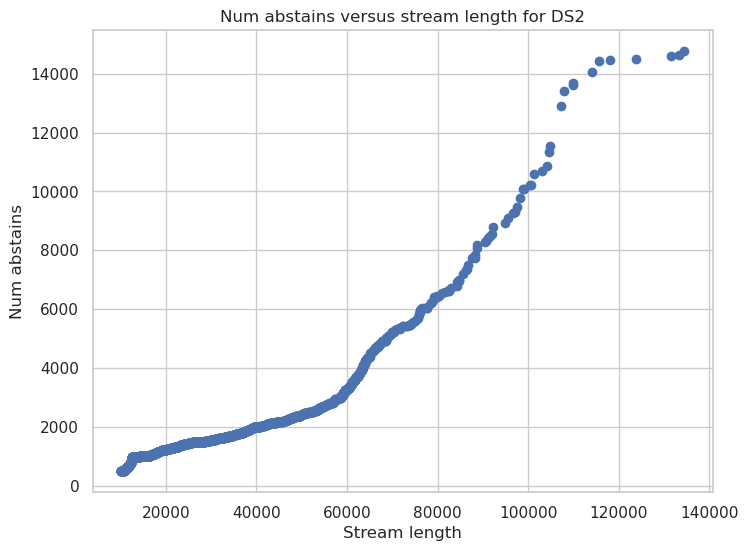
\includegraphics[width=0.7\linewidth]{anomaly/figs/abstain_ds2.png}
    \caption{Number of abstains versus stream length.} 
    \label{fig:abstainsgrowth}
\end{figure}

\paragraph{Contributions} We are the first work to systematically study the problem of unsupervised anomaly thresholding. We propose algorithms in various settings, and provide a principled framework to analyze their performance. Our contributions are: 

\begin{enumerate}
\item {\color{red} Our method provides a statistical framework to tune anomaly thresholds in an online fashion. Our methodology picks a `cold-start' period that is data dependent. Anomalies that are harder to distinguish have a larger cold-start than those that are easier to distinguish.
Thus, our methodology gives a principled generalization of the common heuristic of having a fixed cold-start period. }
    %\item Our algorithm improves upon the manually tuned anomaly thresholding with cold-start period commonly used in practice, and provide an algorithm where abstaining is adaptive and data-dependent.
    \item We prove guarantees on false positive and false negative rates, and number of abstains. {\color{red} 1-2 sentences on the novelty/difficulty}
    \item We prove that our algorithms and guarantees are adaptive to online distribution shifts. {\color{red}1-2 sentences on how we connect the detection delay with the mistake bounds.}
    \item Our algorithms leverages offline data to improve online performance with best of both worlds results: it significantly lowers number of abstains when offline data is available, and reduces to online algorithm when it is not. {\color{red} Our algorithm is the first to rigorously show the best of both worlds for online threshold selection?}
\end{enumerate}

% \begin{figure}
%     \centering
%     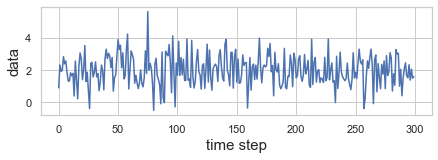
\includegraphics[width=0.9\linewidth]{anomaly/figs/s1.png}
%     \caption{Setting 1, i.i.d. stream}
%     \label{fig:s1}
% \end{figure}


% \begin{figure}
%     \centering
%     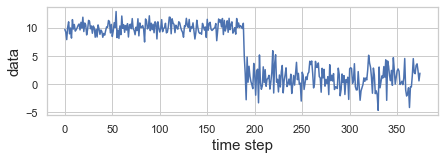
\includegraphics[width=0.9\linewidth]{anomaly/figs/s2.png}
%     \caption{Setting 2, non-stationary stream}
%     \label{fig:s1}
% \end{figure}


% \begin{figure}
%     \centering
%     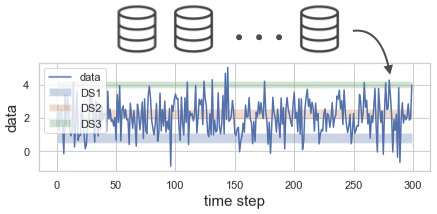
\includegraphics[width=0.9\linewidth]{anomaly/figs/s3.jpeg}
%     \caption{Setting 3, stationary data stream with dataset}
%     \label{fig:s1}
% \end{figure}


\begin{theorem}[Main result of Algorithm \ref{alg:five}] We have online stream $S_1, S_2, \ldots, S_T$  generated from a piece-wise stationary process $\Bigl(T,H_T, (\tau_c)_{c=0}^{H_T}, (f_c)_{c=0}^{H_T}\Bigr)$, and offline datasets  $\gD_1, \ldots, \gD_L$ satisfying the conditions in Theorem \ref{thm:setting_3}. Denote by the online quantile shifts as $\Delta_{k} = \text{Shift} (f_{k},f_{k+1})$. With probability at-least $1-(L+T+1)\alpha$, for all times $T \in \mathbb{N}$, Algorithm \ref{alg:five} satisfies:
\begin{itemize}[noitemsep, topsep=-5pt,labelwidth=!, labelindent=0pt]
    \item  $\text{FP} + \text{FN}  \leq \sum_{k=1}^{H_t}D(\Delta_{k},\alpha)$ 
    \item Number of abstains less than 
    \begin{align*}
        \sum_{k=1}^{H_t} \Bigl[ &(1-\mathbf{1}_{\text{Match}_k}) 4 \sqrt{(\tau_k-\tau_{k-1}) \ln \left( \frac{1612}{\alpha^2} \ln(e(\tau_k-\tau_{k-1})) \right)} \\ & +  D(\Delta_{k},\alpha) \Bigr]
    \end{align*}
\end{itemize}
\label{thm:core_theorem}
\end{theorem}


\subsection{Case study of real AD application}

In addition, we also run Algorithms \ref{alg:two} and \ref{alg:five} on two large scale datasets {\ttfamily DS1} and {\ttfamily DS2} obtained from monitoring two large cloud computing services. Each dataset is a stream of anomaly scores obtained by applying a single anomaly detection algorithm. On these datasets, we run our two general algorithms, Algorithm \ref{alg:two} and \ref{alg:five} with $p = 1 - 10^{-6}$ and $\alpha = 10^{-6}$. Algorithm \ref{alg:five} can use offline datasets. In order to create them, we sampled 50 streams randomly that had length at-least $20,000$ in each of the two datasets. From this collection of $100$ streams, we sub-selected $37$ and $23$ streams from datasets {\ttfamily DS1} and {\ttfamily DS2} respectively such that no two datasets in this collection of $60$ streams overlapped. The description of the rest of the dataset on which we run the online algorithms is in Table \ref{tab:real_data_stats}. In addition, we also run {\ttfamily DSpot} \cite{siffer2017anomaly} with $p = 1 - 10^{-6}$ and set {\ttfamily num-init} to $500$ and {\ttfamily depth} to $100$ on the online algorithm dataset. All other parameters of {\ttfamily DSpot} was set to the suggested values in \cite{siffer2017anomaly}. In addition to these, we also compare against two static baselines of using the first $500$ and $100$ samples respectively and set the threshold as the max of the observed samples. This threshold is not changed since. 

The results of this experiment are reported in Table \ref{tab:real_data}. From this table, we can see that incorporating offline data reduces the number of abstains for both datsets without changing the volume of anomalies raised. This shows that when there are offline datasets available to the algorithm, the online performance is improved. 


\begin{table}[h!]
    \centering
    \resizebox{\columnwidth}{!}{%
    \begin{tabular}{c|c|c|c}
    \toprule
     & Num. of Streams & Average stream length &  Total num samples   \\ \midrule 
{DS1}  & $8377$ & $10925.4$ & $91521785$\\ \midrule
{DS2}  & $9657$ &  $10855.6$ & $104832532$\\
         \bottomrule
    \end{tabular}
    }
    \caption{Real data characteristics}
    \label{tab:real_data_stats}
\end{table}
